% !TeX program = xelatex
% 已同步第三章方法示意圖；接在 3.3 之後。

% ==================================================
% 3.4 動態障礙預測與導航參考調整
% ==================================================
\section{動態障礙預測與導航參考調整}
\label{sec:dynamic_obstacle_avoidance}

動態室內環境中的障礙會隨時間改變可通行空間。本節結合障礙運動估測、候選運動評估與導航參考調整，使控制器在接近障礙前，便能比較不同速度及繞行方向對未來間距與行進進度的影響。調整後的參考再交由全身 GMPC 求解，並透過 CBF、雷射防護與命令放行核對處理運動限制。障礙運動採等速度近似，候選預測則用於有限時間內的運動選擇。

% ==================================================
% 3.4.1 障礙物表示與運動估測
% ==================================================
\subsection{障礙物表示與運動估測}
\label{subsec:obstacle_representation_prediction}

雷射量測先經有效距離與自身回波篩選，再轉換至共同座標系。已知地圖提供固定牆面資訊，其餘候選回波則依掃描角度的相鄰關係形成群集，並與既有軌跡進行資料關聯。群集中心用於追蹤與速度估計；避障幾何則保留物件表面的量測樣本，使較長或不規則的障礙可由多個局部樣本描述。

對第 $g$ 個追蹤物件，定義平面狀態 $x_g=[c_g^{\top},v_g^{\top}]^{\top}\in\mathbb{R}^{4}$，其中 $c_g$ 為追蹤中心，$v_g$ 為平面速度。採用等速度模型與卡爾曼濾波\cite{kalman1960filter}估計其狀態，模型表示為
\begin{equation}
    \begin{aligned}
        x_g^{+}
        &=F_o(\Delta\tau)x_g+w_g, \\
        y_g
        &=H_o x_g+n_g, \\
        F_o(\Delta\tau)
        &=\begin{bmatrix}
            I_2 & \Delta\tau I_2 \\
            \mathbf{0}_{2\times2} & I_2
          \end{bmatrix}, \\
        H_o
        &=\begin{bmatrix}
            I_2 & \mathbf{0}_{2\times2}
          \end{bmatrix},
    \end{aligned}
    \label{eq:ch3_obstacle_tracking_model}
\end{equation}
其中 $\Delta\tau$ 為相鄰追蹤更新的時間間隔，$y_g$ 為群集中心量測，$w_g$ 與 $n_g$ 分別表示程序與量測雜訊。追蹤更新間隔與控制週期 $\Delta t$ 分別處理，避免將不同更新頻率視為相同。

以 $\ell$ 表示送入控制器的障礙幾何樣本，令 $\hat{o}_{\ell,k}\in\mathbb{R}^{2}$ 為其目前估計位置，$\hat{v}_{\ell,k}\in\mathbb{R}^{2}$ 為所屬物件的速度估計。預測時域內的位置為
\begin{equation}
    o_{\ell,i|k}
    =\hat{o}_{\ell,k}+i\Delta t\hat{v}_{\ell,k},
    \qquad i=0,\ldots,N-1.
    \label{eq:ch3_obstacle_cv_prediction}
\end{equation}
同一物件的表面樣本共用其平移速度；已知固定牆面則取零速度。若暫時缺少新觀測，保留的表面樣本依追蹤中心的估計位移平移，使幾何位置與速度對應至相同時刻。此近似未描述物件在遮蔽期間的旋轉與變形，其可保留時間及保護距離依實驗設定。

對直接使用表面回波的樣本，不再重複加入完整物件半徑。若以物件中心及外形半徑表示障礙，則保留對應半徑。兩種表示皆以有效排除距離 $\rho_{\ell}$ 納入後續屏障函數，並透過樣本間距與數量上限控制問題規模。

參考調整層另外將相鄰表面樣本組成障礙群，保留其可見中心的歷史位置。令 $\mu_{g,k}$ 為第 $g$ 群的可見中心，當歷史區間足夠時，由區間位移估計速度，再以一階濾波平滑：
\begin{equation}
    \begin{aligned}
        v_{g,k}^{\mathrm{hist}}
        &=\frac{\mu_{g,k}-\mu_{g,k-r}}{t_k-t_{k-r}},\\
        \tilde v_{g,k}
        &=(1-\lambda_k)\tilde v_{g,k-1}
          +\lambda_k v_{g,k}^{\mathrm{hist}},\\
        \lambda_k&=1-\exp(-\Delta\tau_k/\tau_v).
    \end{aligned}
    \label{eq:ch3_reference_obstacle_velocity}
\end{equation}
其中 $\tau_v>0$ 為平滑時間常數；歷史不足時，以追蹤器速度初始化。此速度供候選運動評估使用，原有 CBF 仍使用其障礙樣本與速度輸入。兩者的資料來源及更新方式分別記錄，避免將新增參考層視為追蹤器本身的替換。


% ==================================================
% 3.4.2 未來相對運動與衝突預測
% ==================================================
\subsection{未來相對運動與衝突預測}
\label{subsec:future_motion_conflict}

令 $T_{\mathrm{pred}}$ 為候選評估時間，$\delta t_{\mathrm{pred}}$ 為取樣間隔，$\tau_j=j\delta t_{\mathrm{pred}}$ 為未來取樣時刻。對距離與速度符合篩選條件的障礙群，以等速度模型預測：
\begin{equation}
    o_g^{\mathrm{ref}}(\tau_j)
    =\tilde c_{g,k}+\tau_j\tilde v_{g,k}.
    \label{eq:ch3_reference_obstacle_prediction}
\end{equation}
其中 $\tilde c_{g,k}$ 為由可見表面中心及外形近似得到的障礙中心。由於雷射通常僅看見物件朝向感測器的一側，參考層依設定的外形半徑補償中心位置，並以底盤尺寸、障礙外形及額外餘量組成排除距離 $\rho_g^{\mathrm{ref}}$。此中心表示供候選評估使用，與 CBF 的表面樣本表示分別處理。

令 $e_k$ 為導航參考視窗的主要平移方向，$v_{\mathrm{nav},k}$ 為由參考路徑長度與時間估計的前進速度。以 $c$ 表示一組速度與偏移候選，其底盤位置近似為
\begin{equation}
    p_B^{(c)}(\tau_j)
    =p_{B,0}+\rho_c v_{\mathrm{nav},k}e_k\tau_j
      +\delta_c(\tau_j)n_c,
    \label{eq:ch3_candidate_base_motion}
\end{equation}
其中 $\rho_c\geq0$ 為速度比例，$n_c$ 為候選偏移方向，$\delta_c$ 為受變化率限制的偏移量。候選包含維持原路徑、調整速度、向行人行進方向的兩側避讓，以及向行人來向偏移等選項。操作階段依任務限制縮減候選，例如抓取期間僅允許維持或降低前進速度。

候選路徑依合成平移速度上限進行弧長重取樣後，與各障礙群在相同未來時刻的位置比較。定義最小預測間距餘量為
\begin{equation}
    D_c=
    \min_{\substack{g\in\mathcal G_k\\j}}
    \left(
      \|p_B^{(c)}(\tau_j)-o_g^{\mathrm{ref}}(\tau_j)\|
      -\rho_g^{\mathrm{ref}}
    \right),
    \label{eq:ch3_candidate_clearance_margin}
\end{equation}
其中 $\mathcal G_k$ 為本次納入的障礙群。側移方向可由主要衝突物件決定，但 $D_c$ 同時考量集合內的其他障礙，以降低避開單一物件卻接近另一物件的情況。此評估使用局部走向與離散取樣近似；實際路徑彎曲、障礙變速與遮蔽的影響，仍需在後續控制與實驗中檢查。

不同候選運動與行人的預測位置如\cref{fig:ch3_dynamic_obstacle_prediction}所示。(a) 為目前觀測，(b) 至 (d) 分別比較原速度、減速與側移在相同未來時刻的位置。減速改變抵達交會區的時間，側移則改變通行位置；實際候選評估依式\eqref{eq:ch3_candidate_clearance_margin}共同考量各障礙與全部選定取樣時刻。

\begin{figure}[htbp]
    \centering
    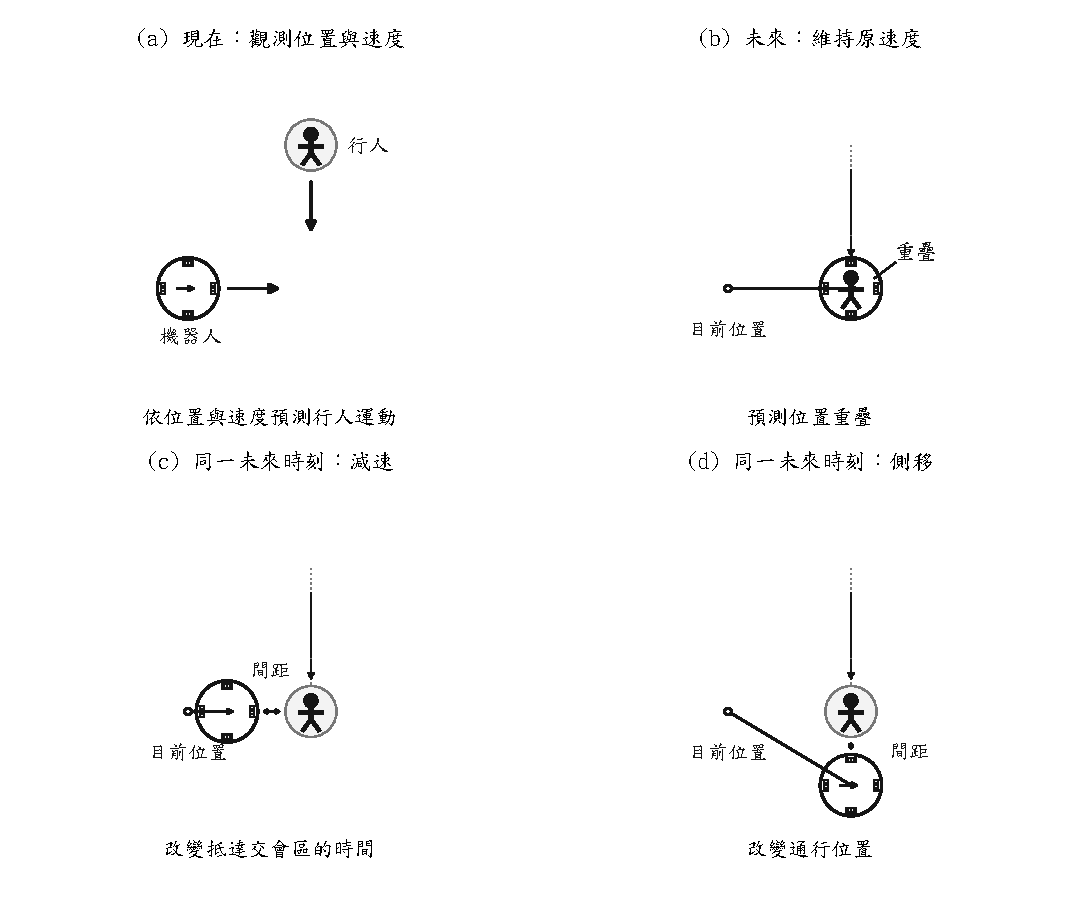
\includegraphics[width=0.98\textwidth]{figsrc/ch03/dynamic_obstacle_prediction.pdf}
    \caption{同一未來時刻下原速度、減速與側移候選之位置比較}
    \label{fig:ch3_dynamic_obstacle_prediction}
\end{figure}

% ==================================================
% 3.4.3 速度與側移候選評估及導航參考更新
% ==================================================
\subsection{速度與側移候選評估及導航參考更新}
\label{subsec:candidate_reference_update}

側移候選先依地圖距離場與最新未知靜態回波進行取樣淨空篩選。對保留的候選，建立進度、偏移與切換成本：
\begin{equation}
    J_c=
    T_{\mathrm{pred}}
    -\frac{e_k^{\top}
       \left(p_B^{(c)}(T_{\mathrm{pred}})-p_{B,0}\right)}
          {v_{\mathrm{nav},k}}
    +w_{\mathrm{lat}}\delta_{c,\max}
    +w_{\mathrm{sw}}\mathbb I(c\ne c_{k-1}),
    \label{eq:ch3_candidate_motion_cost}
\end{equation}
其中 $\delta_{c,\max}$ 為最大偏移量，$\mathbb I(\cdot)$ 為指示函數。第一、二項共同描述相對於原前進速度的進度損失，其餘兩項抑制過大側移與頻繁切換。前進速度過小時不啟用此評估，以避免分母接近零。

令 $\mathcal A_k$ 為經幾何篩選的候選集合，$\mathcal A_k^{+}$ 為預測間距符合要求的子集合，則選擇規則表示為
\begin{equation}
    c_k^{*}=
    \begin{cases}
        \displaystyle\arg\min_{c\in\mathcal A_k^{+}}J_c,
          &\mathcal A_k^{+}\ne\varnothing,\\[1mm]
        \displaystyle\arg\max_{c\in\mathcal A_k}D_c,
          &\mathcal A_k^{+}=\varnothing,\
           \mathcal A_k\ne\varnothing.
    \end{cases}
    \label{eq:ch3_candidate_selection_rule}
\end{equation}
切換至不同候選時，另要求額外間距餘量以形成遲滯。若無候選符合間距要求，則記錄不可行狀態，使用較大最小預測間距的退化選擇，後續仍須接受 CBF、命令限制及放行核對。候選中的零前進速度亦不代表已取得可立即執行的停止命令。

所選速度比例以弧長時間縮放方式作用於原導航參考，側移量則逐步增加或收回。參考位置改變後，對相鄰位姿定義
\begin{equation}
    \begin{aligned}
        \Delta X_{r,i}
        &=X_{r,i}^{-1}X_{r,i+1},\\
        \xi_{r,i}
        &=\frac{1}{\Delta t}
          \begin{bmatrix}
            (\Delta X_{r,i})_{13}\\
            (\Delta X_{r,i})_{23}\\
            \operatorname{atan2}
              ((\Delta X_{r,i})_{21},(\Delta X_{r,i})_{11})
          \end{bmatrix}.
    \end{aligned}
    \label{eq:ch3_reference_velocity_reconstruction}
\end{equation}
此式以相鄰位置差在前一步本體座標中的表示近似平移速度，並以相對航向差計算角速度，使位置參考與速度前饋保持一致。候選評估與實際參考更新使用不同的局部近似，更新後的參考仍由全身控制器重新求解。門區及操作中的啟用範圍，依任務機構與幾何核對配置決定。

% ==================================================
% 3.4.4 控制屏障函數與避障限制
% ==================================================
\subsection{控制屏障函數與避障限制}
\label{subsec:cbf_obstacle_constraints}

控制屏障函數（Control Barrier Function, CBF）可將集合維持需求轉換為控制輸入的條件，其基本理論與控制應用可參照 Ames 等人\cite{ames2019cbf}。本研究以底盤的平面圓盤近似建立距離型屏障函數：
\begin{equation}
    \begin{aligned}
        h_{\ell}(p_B,t)
        &=\|p_B-o_{\ell}(t)\|^2-\rho_{\ell}^{2}, \\
        \rho_{\ell}
        &=r_{\ell}+m_{\ell},
    \end{aligned}
    \label{eq:ch3_obstacle_barrier_function}
\end{equation}
其中 $r_{\ell}$ 為障礙樣本所代表的幾何半徑，$m_{\ell}$ 為包含底盤尺寸與額外間距的保護距離。表面樣本的幾何半徑可取零，其排除距離由保護距離構成。$h_{\ell}\geq0$ 表示底盤中心位於該樣本的排除區域之外。

在保護距離固定、障礙採等速度預測時，沿底盤與障礙運動微分可得
\begin{equation}
    \dot{h}_{\ell}
    =2(p_B-o_{\ell})^{\top}
      \left(R_B(\theta_B)v_B-\hat{v}_{\ell,k}\right),
    \label{eq:ch3_obstacle_barrier_derivative}
\end{equation}
其中 $v_B=[v_x^B,v_y^B]^{\top}$ 為底盤本體座標中的平移速度。選取 $\alpha_h>0$，採用速度型屏障條件
\begin{equation}
    \dot{h}_{\ell}+\alpha_h h_{\ell}
    \geq-\varepsilon_{c(\ell),i|k},
    \qquad \varepsilon_{c(\ell),i|k}\geq0,
    \label{eq:ch3_velocity_cbf_condition}
\end{equation}
其中 $\varepsilon_{c(\ell),i|k}$ 為第 $i$ 個預測時刻的鬆弛變數，$c(\ell)$ 表示該樣本所屬的限制群組。依控制配置，樣本可共用同一組鬆弛，或區分固定幾何與移動障礙的鬆弛，以分別調整其懲罰。

為建立線性限制，第零步使用控制問題起點的底盤位姿，其後各步從底盤誤差模型採用的軌跡取得位置與方向，作為限制條件的評估點。令 $\bar{p}_{B,i|k}$ 與 $\bar{R}_{B,i|k}$ 為該評估點的位置及旋轉矩陣，並定義
\begin{equation}
    \begin{aligned}
        \bar{d}_{\ell,i|k}
        &=\bar{p}_{B,i|k}-o_{\ell,i|k}, \\
        \bar{h}_{\ell,i|k}
        &=\|\bar{d}_{\ell,i|k}\|^2-\rho_{\ell}^{2}, \\
        a_{\ell,i|k}^{\top}
        &=\begin{bmatrix}
            2\bar{d}_{\ell,i|k}^{\top}\bar{R}_{B,i|k} & 0
          \end{bmatrix}.
    \end{aligned}
    \label{eq:ch3_cbf_nominal_geometry}
\end{equation}
將底盤速度命令 $\xi_{B,i|k}=\xi_{r,k+i}+\delta\xi_{i|k}$ 代入，可將式\eqref{eq:ch3_velocity_cbf_condition}整理為
\begin{equation}
    \begin{aligned}
        a_{\ell,i|k}^{\top}\delta\xi_{i|k}
        +\varepsilon_{c(\ell),i|k}
        \geq{}&2\bar{d}_{\ell,i|k}^{\top}\hat{v}_{\ell,k} \\
               &-\alpha_h\bar{h}_{\ell,i|k}
                -a_{\ell,i|k}^{\top}\xi_{r,k+i}.
    \end{aligned}
    \label{eq:ch3_cbf_affine_constraint}
\end{equation}
此限制直接作用於對應步的底盤速度偏差；在全身控制序列中，手臂命令欄補零。角速度欄為零，是因為圓盤距離的一階變化未直接包含偏航速度，底盤航向仍會影響後續運動方向與各步的幾何評估。

將各障礙樣本及選定預測時刻的限制堆疊後，可加入前節的二次規劃問題。令 $\boldsymbol{\varepsilon}_k$ 為全部啟用的鬆弛變數，決策向量擴充為 $\mathbf{z}_{\mathrm{QP},k}=[\mathbf{U}_k^{\top},\boldsymbol{\varepsilon}_k^{\top}]^{\top}$，並於目標函數加入
\begin{equation}
    J_{\varepsilon}
    =\sum_{c\in\mathcal{C}}\sum_{i=0}^{N-1}
      w_{\varepsilon,c,i}\varepsilon_{c,i|k}^{2},
    \qquad w_{\varepsilon,c,i}>0,
    \label{eq:ch3_cbf_slack_cost}
\end{equation}
其中 $\mathcal{C}$ 為啟用的限制群組。當前步與未來步可採不同懲罰權重；提高權重仍屬軟限制，需同時記錄鬆弛量及原始屏障條件的殘差，才能判斷限制的實際滿足程度。

上述限制會隨控制週期重新計算。由於涉及離散更新、幾何近似與鬆弛變數，其實際避障能力需由實驗驗證。本節的平面限制主要描述底盤與障礙的關係，伸展手臂與持物的三維幾何條件則另行處理。

% ==================================================
% 3.4.5 原始雷射掃描防護與命令處理
% ==================================================
\subsection{原始雷射掃描防護與命令處理}
\label{subsec:raw_scan_command_protection}

障礙回波可能因群集大小、資料關聯或運動分類條件而未進入預測控制器。為處理此類情況，底盤命令執行路徑另使用不依賴物件追蹤的雷射防護。量測仍需進行有效距離、自身回波及必要的鄰點一致性篩選。若操作中的門扇另由機構幾何核對處理，則依任務狀態對其回波施加專用遮罩；此類例外須連同啟用條件及恢復時機記錄。

令 $z_{\ell}^{B}\in\mathbb{R}^{2}$ 為轉換至底盤座標的有效回波，$R_{\mathrm{body}}$ 為底盤圓盤近似半徑，定義
\begin{equation}
    \begin{aligned}
        n_{\ell}
        &=\frac{z_{\ell}^{B}}{\|z_{\ell}^{B}\|}, \\
        d_{\ell}
        &=\|z_{\ell}^{B}\|-R_{\mathrm{body}}, \\
        r_{\ell}^{B}
        &=R_{\mathrm{body}}n_{\ell}.
    \end{aligned}
    \label{eq:ch3_scan_surface_geometry}
\end{equation}
其中 $n_{\ell}$ 指向回波，$d_{\ell}$ 為回波至底盤表面的近似間距，$r_{\ell}^{B}$ 為面向回波的底盤表面點。令 $J_2=\begin{bmatrix}0&-1\\1&0\end{bmatrix}$，表面點朝向回波的接近速度為
\begin{equation}
    \begin{aligned}
        v_{n,\ell}
        &=a_{\ell}^{\mathrm{sh}\,\top}\xi_B, \\
        a_{\ell}^{\mathrm{sh}\,\top}
        &=\begin{bmatrix}
            n_{\ell}^{\top} & n_{\ell}^{\top}J_2r_{\ell}^{B}
          \end{bmatrix}.
    \end{aligned}
    \label{eq:ch3_scan_approach_velocity}
\end{equation}
此處 $v_{n,\ell}>0$ 表示底盤表面朝向回波運動。採用圓盤近似時，$n_{\ell}^{\top}J_2r_{\ell}^{B}=0$；此幾何亦說明該防護未直接涵蓋伸展手臂的旋轉掃掠範圍。

以進入防護層的底盤命令 $\xi_B^{\mathrm{in}}$ 計算各點的接近速度，建立所需保護間距：
\begin{equation}
    \begin{aligned}
        v_{\mathrm{app},\ell}
        &=\max\!\left(0,
          a_{\ell}^{\mathrm{sh}\,\top}\xi_B^{\mathrm{in}}\right), \\
        d_{\mathrm{stop},\ell}
        &=d_0+v_{\mathrm{app},\ell}(\tau_0+t_{\mathrm{age}}) \\
        &\quad+\frac{v_{\mathrm{app},\ell}^{2}}{2a_{\mathrm{brake}}}
          +\epsilon_{\mathrm{scan}}+\epsilon_{\mathrm{body}}.
    \end{aligned}
    \label{eq:ch3_scan_stopping_distance}
\end{equation}
其中 $d_0$ 為低速時的基本間距，$\tau_0$ 為延遲裕度，$t_{\mathrm{age}}$ 為距最近一次有效掃描更新的時間，$a_{\mathrm{brake}}>0$ 為採用的減速能力參數，$\epsilon_{\mathrm{scan}}$ 與 $\epsilon_{\mathrm{body}}$ 分別為量測與外形近似裕度。保護間距依各回波方向的接近速度計算，避免以總平移速度將切向通行的間距一併放大。

防護層對輸出命令施加
\begin{equation}
    a_{\ell}^{\mathrm{sh}\,\top}\xi_B^{\mathrm{out}}
    \leq\alpha_{\mathrm{sh}}
          (d_{\ell}-d_{\mathrm{stop},\ell}),
    \qquad \alpha_{\mathrm{sh}}>0,
    \label{eq:ch3_scan_protection_constraint}
\end{equation}
並與底盤速度框及啟用的輪級限制共同處理。將全部半空間限制寫成 $A_{\mathrm{sh}}\xi_B\leq b_{\mathrm{sh}}$，由輸入命令開始，反覆選取違反量最大的限制列進行投影。若該列為 $a_j^{\top}\xi_B\leq b_j$，則更新式為
\begin{equation}
    \xi_B^{(n+1)}
    =\xi_B^{(n)}
     -\frac{\left[a_j^{\top}\xi_B^{(n)}-b_j\right]_{+}}
            {\|a_j\|^2}a_j,
    \label{eq:ch3_scan_halfspace_projection}
\end{equation}
其中 $[x]_{+}=\max(x,0)$。投影採有限迭代預算，完成後檢查限制殘差；迭代次數本身不代表限制已全部滿足。

若完整防護條件仍無法滿足，則先將要求主動退離的負上界放寬至零，形成該方向的非接近條件，再進行投影與殘差核對。若仍無法取得合格命令，則進入停止請求與輪級減速處理。當輪級命令變化限制同時作用時，零速度請求未必能立即執行，因此仍需核對最終放行命令。掃描更新逾時則進入低速退化處理，此時不能將缺少新回波解讀為環境無障礙。

底盤命令依序經過速度平滑、雷射防護及最終輪級限制，再送至底盤執行介面。防護層以最近的最終放行命令作為輪級變化限制的基準，並記錄回退來源與命令修正量。若後處理改變原本的最佳化命令，其對底盤與末端預測的影響，需配合執行端回報於後續控制週期處理，相關方法於執行動態補償一節說明。

上述雷射防護用於抑制機器人對可見回波的接近運動，未直接估測回波所屬障礙的速度，因此需與前述動態障礙預測配合。其效能與適用範圍，於第四章依避障距離、命令修正及任務表現進行評估。

% ==================================================
% 3.4.5 導航參考調整、預測避障與底盤命令處理之分層關係
% ==================================================
各層的作用位置如\cref{fig:ch3_navigation_command_layers}所示。參考調整改變導航目標序列，CBF 作用於全身最佳化問題，雷射防護與輪級限制則依序處理待執行底盤命令；最終放行值回報後，供後續命令限制與運動預測使用。

\begin{figure}[htbp]
    \centering
    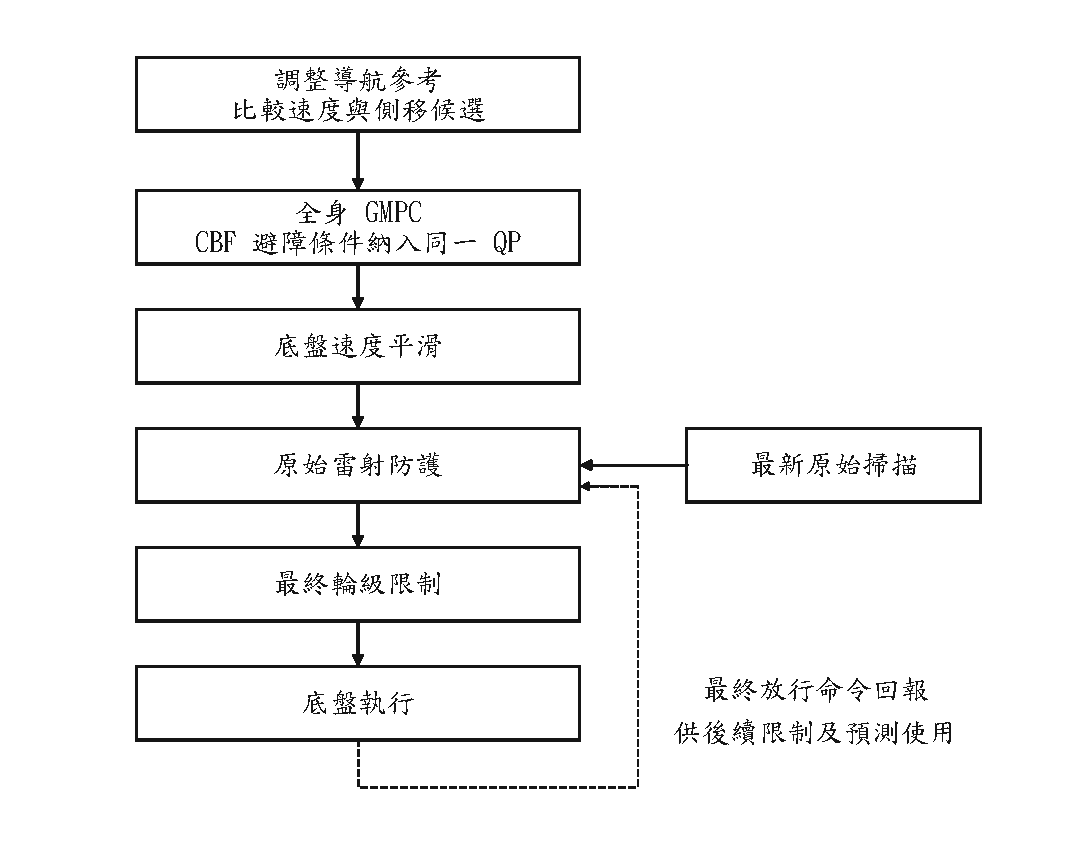
\includegraphics[width=0.98\textwidth]{figsrc/ch03/navigation_command_layers.pdf}
    \caption{導航參考調整、預測避障與底盤命令處理之分層關係}
    \label{fig:ch3_navigation_command_layers}
\end{figure}

% ==================================================
% 3.5 視覺目標估測與任務參考生成
% ==================================================
\section{視覺目標估測與任務參考生成}
\label{sec:visual_task_reference}

移動操作所需的參考包含物件位置、抓取方向、底盤接近位置及操作進度。Mittal 等人\cite{mittal2022articulated}將 RGB-D 感知、物件操作規劃與全身控制整合，呈現感知資訊與操作模型銜接的重要性。本研究以已知類型的門把手、抽屜把手、圓柱及筆狀代理物為對象，利用深度幾何估測更新操作目標，再依導航可達性與手臂構型產生控制參考。


% ==================================================
% 3.5.1 任務目標之視覺定位與幾何估測
% ==================================================
\subsection{任務目標之視覺定位與幾何估測}
\label{subsec:visual_geometric_estimation}

令深度影像中像素座標為 $(u,v)$，其光軸深度為 $z(u,v)$，相機內參矩陣為 $K_C$。有效深度點在相機座標中的位置為
\begin{equation}
    {}^{C}p(u,v)
    =z(u,v)K_C^{-1}
      \begin{bmatrix}u&v&1\end{bmatrix}^{\top}.
    \label{eq:ch3_depth_backprojection}
\end{equation}
量測先經距離與任務區域篩選，再依目標類型估計幾何。家具登錄位置用於限制搜尋範圍，精確操作目標由當次有效觀測修正；物件尺寸、家具外形與機構軸向等已知資訊則作為先驗。

抽屜把手以面板點群估計櫃面方向，再由面板前方的橫桿點群取得桿心與高度。門扇開度則由鉸鏈附近的點群主方向估計，並核對可見長度及擬合直線與鉸鏈的距離。筆狀物件以點群主成分取得長軸方向，再利用長寬條件與頂面點估計中心。

對已知半徑 $r_o$ 的直立圓柱，令 $P_\ell^{xy}$ 為候選側面點的水平投影，以可見點群中心及半徑補償建立初值，再求解
\begin{equation}
    \hat c_o=
    \underset{c\in\mathbb R^2}{\operatorname{arg\,min}}
    \sum_{\ell}
    \left(\|P_\ell^{xy}-c\|-r_o\right)^2.
    \label{eq:ch3_known_radius_object_fit}
\end{equation}
式中以高斯牛頓法由初值迭代取得局部解。圓柱中心高度依桌面高度與已知物件高度建立，繞對稱軸的方向則由抓取需求選擇。筆狀物件的主軸具有 $\pi$ 方向歧義，需由可行抓取構型選擇對應方向。上述估測只輸出各物件可觀測且任務所需的幾何量，其餘分量由已知模型與操作條件決定。


% ==================================================
% 3.5.2 影像、機器人狀態與座標轉換之時間對齊
% ==================================================
\subsection{影像、機器人狀態與座標轉換之時間對齊}
\label{subsec:visual_state_time_alignment}

機器人在影像取得與控制求解之間可能持續移動，因此，目標轉換須使用影像觀測時刻的相機位姿。令 $t_o$ 為觀測時間，世界座標中的量測點為
\begin{equation}
    \begin{bmatrix}{}^{W}p\\1\end{bmatrix}
    ={}^{W}T_C(t_o)
      \begin{bmatrix}{}^{C}p\\1\end{bmatrix},
    \qquad
    {}^{W}T_C(t_o)
    ={}^{W}T_B(t_o)\,{}^{B}T_C(q_a(t_o)).
    \label{eq:ch3_visual_timestamp_transform}
\end{equation}
對固定於底盤的相機，$ {}^{B}T_C$ 為固定外參；對手腕相機，則包含手臂運動鏈與相機安裝偏移。使用平台狀態與模型外參時，須保留其座標定義及來源時間。

目標封包保留觀測時間、座標系、估計幾何與有效性資訊。影像處理完成後仍沿用原觀測時間，並在接近或抓持前檢查資料新鮮度、可見點數與幾何一致性。對暫時遮蔽的目標，可在既定有效時間內保留估計；超過條件時重新觀測或停止該階段的推進。

底盤相機與手腕相機依可見性及任務階段提供觀測。當次實驗使用的來源、更新時機及保留策略分別記錄，避免將不同來源的結果視為同一時刻的量測。

% ==================================================
% 3.5.2 視覺量測與相機位姿依觀測時間配對之流程
% ==================================================
視覺量測與相機位姿的時間配對如\cref{fig:ch3_visual_time_alignment}所示。影像處理完成後仍保留原觀測時間 $t_o$，並使用該時刻的相機位姿進行座標轉換，再將世界座標中的目標提供給操作參考生成。

\begin{figure}[htbp]
    \centering
    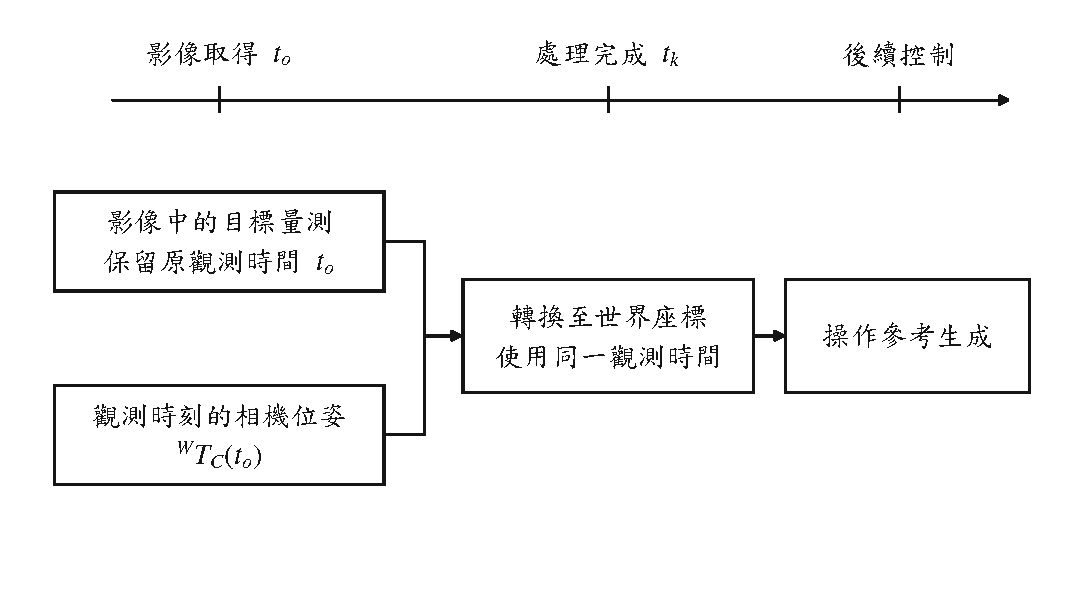
\includegraphics[width=0.98\textwidth]{figsrc/ch03/visual_time_alignment.pdf}
    \caption{視覺量測與相機位姿依觀測時間配對之流程}
    \label{fig:ch3_visual_time_alignment}
\end{figure}

% ==================================================
% 3.5.3 可行操作區域與底盤目標選擇
% ==================================================
\subsection{可行操作區域與底盤目標選擇}
\label{subsec:feasible_operation_base_selection}

操作目標確定後，需選擇可由導航到達、且手臂能完成接近與抓持的底盤位置。候選由目標與家具幾何生成，再檢查底盤淨空、最新未知障礙點、關節限制、預抓與抓取構型，以及相關路段的可達性。

以圓柱物件的候選評分為例，令 $\mathcal F_k$ 為本次通過檢查的有限候選集合，採用
\begin{equation}
    (b^{*},q_a^{*})
    =\underset{(b,q_a)\in\mathcal F_k}{\operatorname{arg\,min}}
      \left[
        w_L L_{\mathrm{route}}(b)
        +\frac{w_\sigma}
         {\max(\sigma_{\min}(J_{\mathrm{sel}}(q_a)),\epsilon_\sigma)}
      \right],
    \label{eq:ch3_operation_base_selection}
\end{equation}
其中 $b=[x_B,y_B,\theta_B]^{\top}$，$L_{\mathrm{route}}$ 為路線長度估計，$J_{\mathrm{sel}}$ 為選位評估使用的手臂雅可比，$\epsilon_\sigma>0$ 用於避免分母接近零。啟用格點路線評估時，由已知家具及未知回波建立可行域，並以 Dijkstra 最短路徑方法\cite{dijkstra1959note}取得路線成本。不同任務可依後續目標及朝向增加評分項。

選定候選提供導航目標、操作朝向與可用構型，實際接近路徑仍由導航前端更新。候選區域與路線需配合新觀測重新核對；式\eqref{eq:ch3_operation_base_selection}的選擇範圍為當次已生成且已檢查的候選集合。

底盤選位前後的操作關係如\cref{fig:ch3_visual_operation_reference}所示。系統依已定位目標與家具幾何產生底盤候選，通過淨空、路線與手臂構型檢查後，再依評分選擇操作位姿。選定結果提供導航接近目標與可用手臂構型，後續仍依實際狀態更新控制參考。

\begin{figure}[htbp]
    \centering
    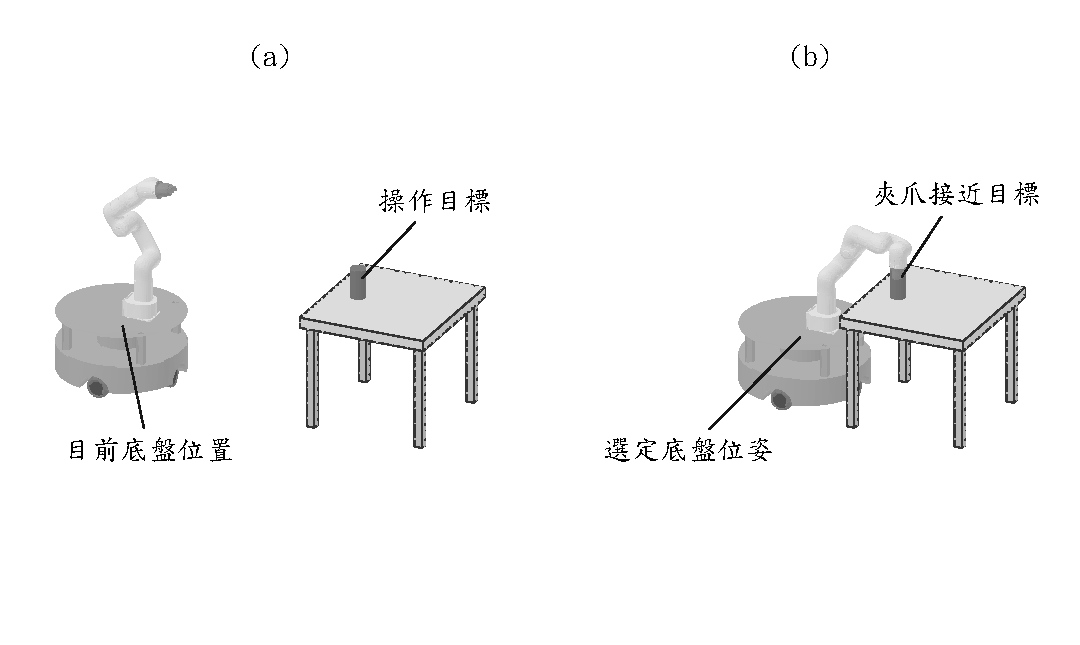
\includegraphics[width=0.98\textwidth]{figsrc/ch03/visual_operation_reference.pdf}
    \caption{操作目標導引之底盤選位與手臂接近}
    \label{fig:ch3_visual_operation_reference}
\end{figure}

% ==================================================
% 3.5.4 導航路徑下之朝向與末端參考生成
% ==================================================
\subsection{導航路徑下之朝向與末端參考生成}
\label{subsec:navigation_manipulation_reference}

移動中接近時，底盤平移參考沿用導航前端提供的路徑，操作端依剩餘距離調整朝向、速度上限與末端展開進度。令 $\theta_{\mathrm{nav},i}$ 為導航朝向，$\theta_g$ 為操作朝向，則以距離權重 $w_i\in[0,1]$ 建立
\begin{equation}
    \theta_{r,i}
    =\theta_{\mathrm{nav},i}
     +w_i\operatorname{wrap}
       (\theta_g-\theta_{\mathrm{nav},i}),
    \label{eq:ch3_operation_heading_reference}
\end{equation}
其中 $\operatorname{wrap}(\cdot)$ 將角度差映射至 $(-\pi,\pi]$。接近操作區域時逐步增加 $w_i$，物件抬升並離開抓取階段後，再依任務條件交回導航朝向。

末端展開採用五次平滑函數 $\psi(\nu)=10\nu^3-15\nu^4+6\nu^5$；此函數對應固定端點且端點速度與加速度為零的最小急動軌跡\cite{flash1985coordination}。令 $d_i$ 為參考底盤至操作位置的距離，定義
\begin{equation}
    \nu_i=
    \operatorname{clip}
      \left(\frac{d_{\mathrm{out}}-d_i}
      {d_{\mathrm{out}}-d_{\mathrm{in}}},0,1\right),
    \qquad \beta_i=\psi(\nu_i).
    \label{eq:ch3_distance_based_arm_progress}
\end{equation}
預測進度另依目前進度與最短展開時間限制其增加速度。令 $(p_{\mathrm{rel},i},R_{\mathrm{rel},i})$ 為起始相對構型隨底盤移動所形成的世界位姿，$(p_{\mathrm{line},i},R_{\mathrm{line},i})$ 為預抓或抓取接近線上的目標，則
\begin{equation}
    \begin{aligned}
        p_{E,i}^{d}
        &=(1-\beta_i)p_{\mathrm{rel},i}
          +\beta_i p_{\mathrm{line},i},\\
        R_{E,i}^{d}
        &=R_{\mathrm{rel},i}
          \exp\!\left(
            \beta_i\log(R_{\mathrm{rel},i}^{\top}R_{\mathrm{line},i})
          \right).
    \end{aligned}
    \label{eq:ch3_continuous_approach_reference}
\end{equation}
最後接近線的推進另由底盤位置與 TCP 到位狀態觸發。若導航因避障而改變進度，手臂展開亦隨距離與狀態更新。朝向或位置參考變更後，依式\eqref{eq:ch3_reference_velocity_reconstruction}重新計算底盤參考速度，再建立末端追蹤與命令限制。

% ==================================================
% 3.6 移動中操作與機構約束控制
% ==================================================
\section{移動中操作與機構約束控制}
\label{sec:mobile_constrained_operation}

移動中操作需要協調底盤進度、末端追蹤與物件互動。Burgess-Limerick 等人\cite{burgess2023motm}以移動與操作重疊改善多步驟任務的執行效率；對門與抽屜等關節式物件，則需進一步考量機構運動與全身構型的相容性\cite{mittal2022articulated}。本節以共用全身控制核心承接不同任務參考，說明抓持條件、機構約束及持物狀態的切換。


% ==================================================
% 3.6.1 移動中接近與抓持條件
% ==================================================
\subsection{移動中接近與抓持條件}
\label{subsec:moving_approach_grasp}

物件尚未抓持時，末端目標以世界座標表示。即使底盤持續移動，手臂仍需配合補償底盤造成的相對位移，使 TCP 接近物件。抓取階段依物件外形設定位置容許區域、姿態誤差及適用的相對速度條件；固定橫桿把手另檢查沿夾爪開合軸的誤差。

閉爪時機由接近進度與狀態判定，抓持成立則需持續取得符合條件的手指位置與接觸證據。以 $\gamma_f(t)\in\{0,1\}$ 表示該任務的抓持證據判定，要求
\begin{equation}
    \gamma_f(t)=1,
    \qquad
    t\in[t_b-T_{\mathrm{ev}},t_b],
    \label{eq:ch3_grasp_evidence_duration}
\end{equation}
其中 $T_{\mathrm{ev}}$ 為確認時間，$t_b$ 為判定成立時刻。手指位置、接觸力及持續時間的門檻依物件類型設定，並於第四章揭露。移動中抓取另受可達時間窗約束，錯過時依既定策略重新接近或轉為收斂抓取，並記錄原移動中操作未完成的原因。

目前模擬在抓持證據成立後，依任務使用夾爪與物件間的理想固定連接。連接建立與解除皆由執行端回報確認，控制器再更新抓持狀態。此假設用於研究抓持後的協同運動，其影響於第四章的限制分析說明。

% ==================================================
% 3.6.1 接近、閉爪確認與抓持成立之狀態轉移
% ==================================================
抓持狀態的轉移如\cref{fig:ch3_grasp_state_transition}所示。閉爪命令發出後，需檢查手指位置與接觸證據，待條件持續成立並取得必要的連接確認後，才銜接抓持後的機構操作或持物運送。

\begin{figure}[htbp]
    \centering
    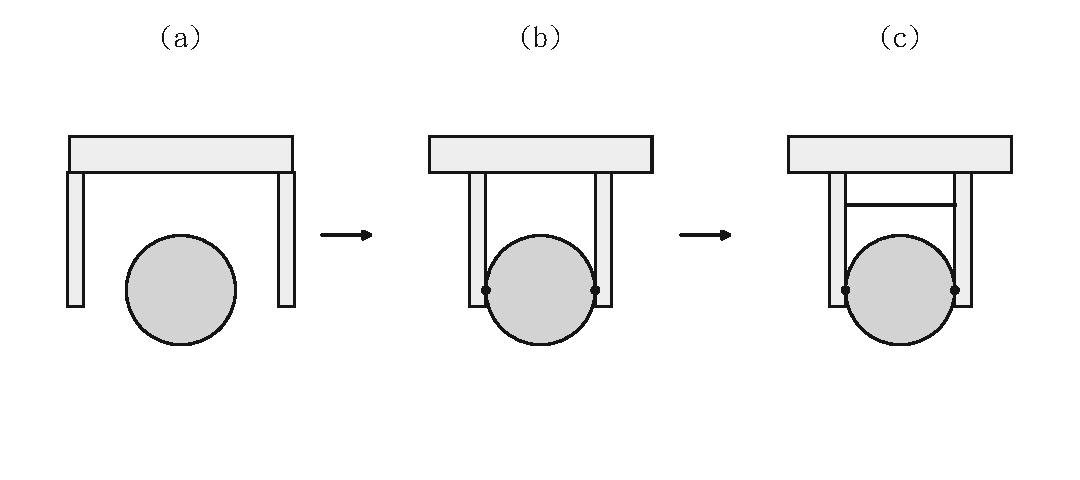
\includegraphics[width=0.98\textwidth]{figsrc/ch03/grasp_state_transition.pdf}
    \caption{接近、閉爪確認與抓持成立之狀態轉移}
    \label{fig:ch3_grasp_state_transition}
\end{figure}

% ==================================================
% 3.6.2 門與抽屜之機構約束建模
% ==================================================
\subsection{門與抽屜之機構約束建模}
\label{subsec:articulated_object_constraints}

令 $\eta$ 為被操作物件的機構座標，$ {}^{W}T_H(\eta)$ 為把手位姿。抓持成立時，由當下物件估計與機器人實測構型建立固定抓持變換：
\begin{equation}
    \begin{aligned}
        {}^{H}T_E
        &=\left({}^{W}T_H(\eta_b)\right)^{-1}
          {}^{W}T_E(\chi_b),\\
        {}^{W}T_E(\chi)
        &={}^{W}T_H(\eta)\,{}^{H}T_E.
    \end{aligned}
    \label{eq:ch3_grasp_closed_chain}
\end{equation}
其中 $\chi_b$ 與 $\eta_b$ 為綁定時刻的構型及機構座標。第二式為抓持後的閉鏈相容關係，底盤與手臂需共同維持末端相對把手的位姿。

對旋轉門，令 $h$ 為鉸鏈軸上一點，$a_h$ 為世界座標中的單位旋轉軸，其方向依門角正向定義。由起始門角 $\phi_0$ 對應的把手位姿，可得
\begin{equation}
    \begin{aligned}
        p_H(\phi)
        &=h+R_{a_h}(\phi-\phi_0)(p_{H,0}-h),\\
        R_H(\phi)
        &=R_{a_h}(\phi-\phi_0)R_{H,0}.
    \end{aligned}
    \label{eq:ch3_revolute_handle_model}
\end{equation}
其中 $R_{a_h}$ 為繞軸 $a_h$ 的旋轉矩陣。開門與關門分別依目標門角更新參考；回程操作前重新估計門扇開度，以處理放手後的門角變化。

% ==================================================
% 3.6.2 開門前後之門扇、底盤與手臂構型
% ==================================================
不同門角下的協同構型如\cref{fig:ch3_door_operation_sequence}所示。把手繞鉸鏈運動時，底盤位置與手臂構型配合調整，並維持式\eqref{eq:ch3_grasp_closed_chain}所定義的抓持相對位姿。

\begin{figure}[htbp]
    \centering
    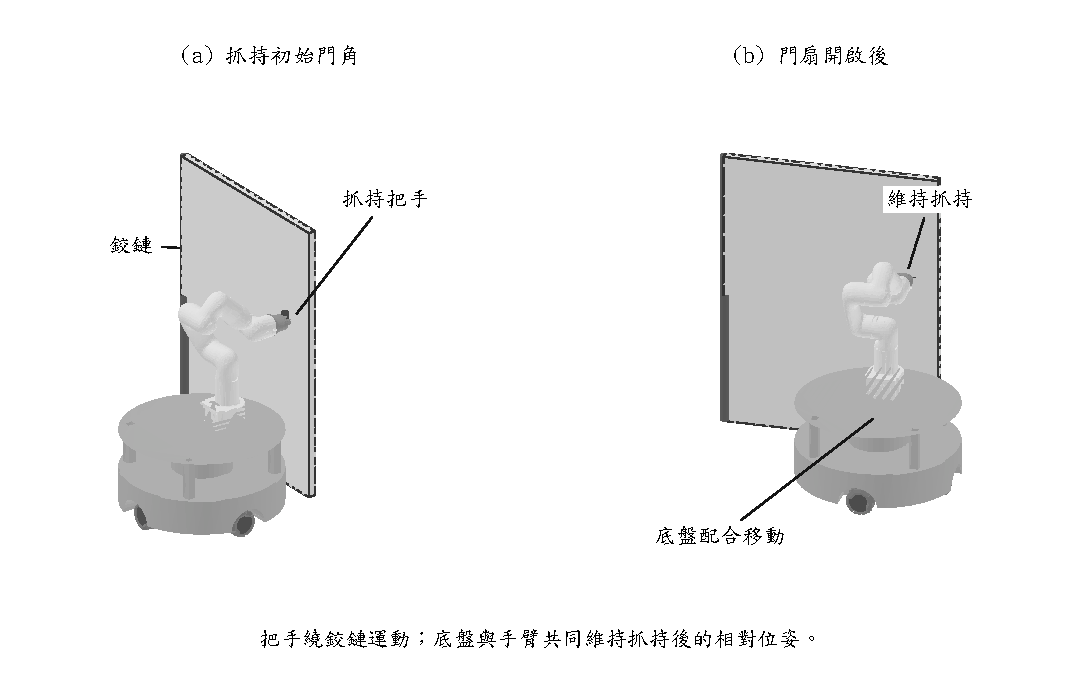
\includegraphics[width=0.98\textwidth]{figsrc/ch03/door_operation_sequence.pdf}
    \caption{開門前後之門扇、底盤與手臂構型}
    \label{fig:ch3_door_operation_sequence}
\end{figure}

對平移抽屜，令 $a_d$ 為拉出方向，$d$ 為相對初始位置的位移，則
\begin{equation}
    p_H(d)=p_{H,0}+d a_d,
    \qquad R_H(d)=R_{H,0}.
    \label{eq:ch3_prismatic_handle_model}
\end{equation}
拉開與推回依位移參考的方向處理，並共同更新底盤與末端參考。物件機構參數、有效行程及家具幾何屬於已知模型或觀測後更新的資訊，實驗中分別揭露其來源。

% ==================================================
% 3.6.2 抽屜拉出前後之滑軌位移與全身構型
% ==================================================
抽屜拉出前後的機構位移與全身構型如\cref{fig:ch3_drawer_operation_sequence}所示。抽屜沿滑軌平移並保持機構姿態，底盤與手臂則依操作進度更新參考，以維持抓持及所需的運動空間。

\begin{figure}[htbp]
    \centering
    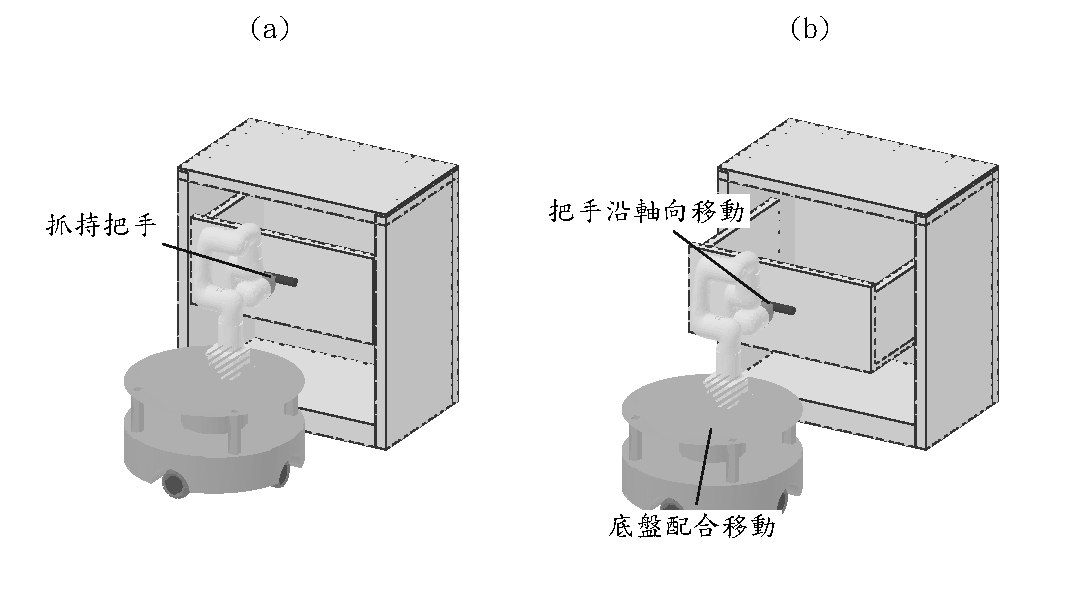
\includegraphics[width=0.98\textwidth]{figsrc/ch03/drawer_operation_sequence.pdf}
    \caption{抽屜拉出前後之滑軌位移與全身構型}
    \label{fig:ch3_drawer_operation_sequence}
\end{figure}



開門階段以把手機構產生末端目標，並可在選定預測步加入閉鏈位姿容許範圍。沿用式\eqref{eq:ch3_tcp_affine_residual}的局部近似，限制為
\begin{equation}
    -\epsilon_c
    \leq r_{0,i|k}-L_{i,k}\mathbf U_k
    \leq\epsilon_c,
    \qquad i\in\mathcal I_c,
    \label{eq:ch3_contact_pose_tube}
\end{equation}
其中 $\epsilon_c$ 分別包含位置與姿態各分量的容許量，$\mathcal I_c$ 為啟用的預測步集合。此限制與底盤、手臂的輸入共同出現在同一 QP 中。

各操作階段依配置採用機構相容參考、QP 限制及執行端幾何核對。抽屜平移與共轉關門的限制實現方式分別說明，不將所有階段視為啟用相同的硬限制。轉動門扇及被操作物件的回波例外，須與專用機構、環境淨空檢查共同啟用，並記錄其適用範圍。


% ==================================================
% 3.6.3 持物運送與收納之運動參考
% ==================================================
\subsection{持物運送與收納之運動參考}
\label{subsec:carrying_storage_reference}

物件抓持成立後，操作目標可由世界固定改為相對底盤的抬升與保持。令 $ {}^{B}T_E^{d}$ 為相對底盤的目標，則其世界位姿為
\begin{equation}
    {}^{W}T_E^{d}
    ={}^{W}T_B\,{}^{B}T_E^{d},
    \qquad
    {}^{B}T_E(q_a)
    ={}^{B}T_A\,{}^{A}T_E(q_a).
    \label{eq:ch3_base_relative_carry_target}
\end{equation}
在相對模式中，追蹤殘差直接由 $ {}^{B}T_E(q_a)$ 與 $ {}^{B}T_E^{d}$ 計算。由於目標與實際末端皆隨底盤作相同剛體運動，其對底盤誤差的局部微分相互抵消，對增廣狀態的幾何映射為
\begin{equation}
    \mathcal J_{E,i}^{\mathrm{rel}}
    =
    \begin{bmatrix}
        \mathbf 0_{6\times3}
        &{}^{B}J_{A,i}
        &\mathbf 0_{6\times6}
    \end{bmatrix}.
    \label{eq:ch3_relative_task_augmented_jacobian}
\end{equation}
因此，持物任務以相對構型維持物件位置，導航則繼續調整底盤運動。相對模式的殘差與雅可比需共同更新，以符合式\eqref{eq:ch3_base_relative_carry_target}的座標關係。

抬升、退出家具、移至收納區及收臂依階段產生參考，並檢查手臂、持物與家具的淨空。當物件放入收納區時，先確認連接解除與釋放狀態，再轉入空手收臂或後續操作。不同實驗採用直接持物返回或先收納再返回時，依各自流程評估。

% ==================================================
% 3.6.3 相對底盤目標下之持物運送與構型保持
% ==================================================
相對底盤目標下的運送關係如\cref{fig:ch3_base_relative_carrying}所示。手臂維持相對底盤的末端構型時，物件在世界座標中的位置隨底盤一起改變。此關係由式\eqref{eq:ch3_base_relative_carry_target}建立，與前述世界固定操作目標分別處理。

\begin{figure}[htbp]
    \centering
    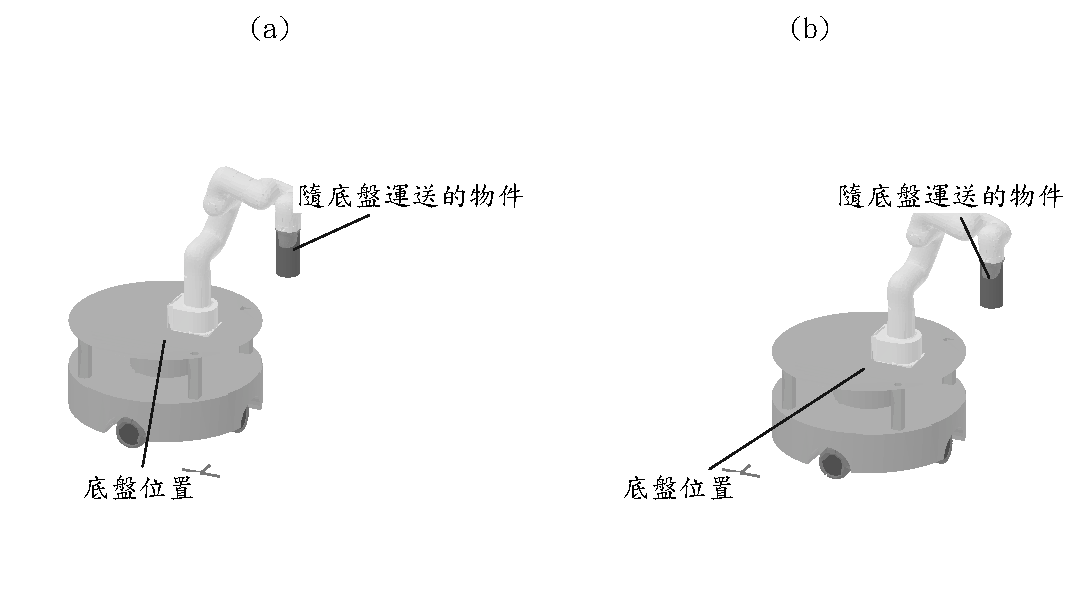
\includegraphics[width=0.98\textwidth]{figsrc/ch03/base_relative_carrying.pdf}
    \caption{相對底盤目標下之持物運送與構型保持}
    \label{fig:ch3_base_relative_carrying}
\end{figure}

% ==================================================
% 3.6.4 任務階段切換與控制狀態延續
% ==================================================
\subsection{任務階段切換與控制狀態延續}
\label{subsec:task_transition_continuity}

任務層管理導航、接近、閉爪確認、機構操作、退出、通行、取物與返回等階段，各階段更新底盤參考、末端目標、權重與啟用限制。轉移條件依觀測、位姿誤差、抓持證據、機構進度及執行端回報判定；時間條件用於軌跡參數化、確認區間及逾時處置。

切換時承接實際關節位置、位置設定點、在途命令、最近放行輸入及模型偏置，並保留可沿用的初始控制序列。新的接近參考由切換時實際相對位姿建立；抓持成立後再依式\eqref{eq:ch3_grasp_closed_chain}建立機構關係。狀態延續使各任務可使用共用全身控制核心，同時維持實際命令的時間順序。

當新階段尚未取得有效目標或未通過交接檢查時，執行端依目前已接受的控制段與停止備援處理。任務切換、求解接受與實際生效分別記錄，以供第四章分析動作接續與非必要等待。

% ==================================================
% 3.7 執行動態補償與控制實現
% ==================================================
\section{執行動態補償與控制實現}
\label{sec:execution_compensation}

前述最佳化以指定初始狀態與未來參考建立控制序列，實際運動則受到命令延遲、設定點追蹤與執行端修正影響。本節整合在途命令前推、模型偏置估測及末端目標補償，並說明控制段放行、非阻塞計算與停止備援，使預測所用狀態與實際執行順序相互對應。


% ==================================================
% 3.7.1 在途命令與實際放行輸入之預測整合
% ==================================================
\subsection{在途命令與實際放行輸入之預測整合}
\label{subsec:queued_applied_command_prediction}

令 $z_k^{\mathrm{ex}}=[\chi_k^{\top},s_{a,k}^{\top}]^{\top}$ 為執行端狀態，包含底盤位姿、實際關節位置與位置設定點。定義完整命令 $v=[\xi_B^{\top},u_a^{\top}]^{\top}$，其底盤分量為實際速度命令，與最佳化中的速度偏差 $\delta\xi$ 分別表示。

新命令生效前，已提交的控制段與通訊管線仍會繼續作用。令 $D_k$ 為新控制段生效前已排定的物理步數，$\mathcal Q_k=\{v_{0|k}^{\mathrm{fix}},\ldots,v_{D_k-1|k}^{\mathrm{fix}}\}$ 為該區間的既定命令。以物理步模型 $f_p$ 依序前推：
\begin{equation}
    \begin{aligned}
        z_{0|k}^{\mathrm{ex}}&=z_k^{\mathrm{ex}},\\
        z_{\ell+1|k}^{\mathrm{ex}}
        &=f_p(z_{\ell|k}^{\mathrm{ex}},v_{\ell|k}^{\mathrm{fix}}),
          \quad \ell=0,\ldots,D_k-1,\\
        t_k^{\mathrm{eff}}&=t_k+D_k\Delta t_p.
    \end{aligned}
    \label{eq:ch3_queued_command_forward_prediction}
\end{equation}
其中 $f_p$ 結合底盤本體速度運動與式\eqref{eq:ch3_physics_step_arm_model}的設定點追蹤關係；既定命令需包含該區間已排定的平滑、斜坡及限制處理。若未來修正尚未知，則於實際放行後以回報命令及新狀態修正下一次預測。

由前推結果建立求解初始狀態：
\begin{equation}
    \zeta_{0|k}=
    \begin{bmatrix}
        \left[
          \log\left(X_r(t_k^{\mathrm{eff}})^{-1}
                    X_{B,D_k|k}\right)
        \right]^{\vee}\\
        q_{a,D_k|k}\\
        s_{a,D_k|k}
    \end{bmatrix}.
    \label{eq:ch3_delay_compensated_initial_state}
\end{equation}
任務參考亦由 $t_k^{\mathrm{eff}}$ 起算，首步命令差分使用該起點之前的生效命令。如此可保留在途命令尚未作用完畢的影響，避免以目前狀態搭配未來生效時刻的命令進行不一致的預測。

底盤命令經防護與輪級限制後，執行端回報最終放行值；手臂則回報實際位置設定點與關節位置。前者更新命令差分及執行紀錄，後者維持增廣模型中 $q_a$ 與 $s_a$ 的區分。各資料以來源時間與序號管理，障礙及視覺資訊另依其有效時間判定。

控制計算與命令接續的時序如\cref{fig:ch3_command_execution_timeline}所示。計算期間既定命令持續執行，控制器依其作用預測新控制段生效時刻的狀態。新結果通過期限與可行性核對後才接續執行；若拒絕或逾時，則沿已核對的停止尾段減速。

\begin{figure}[htbp]
    \centering
    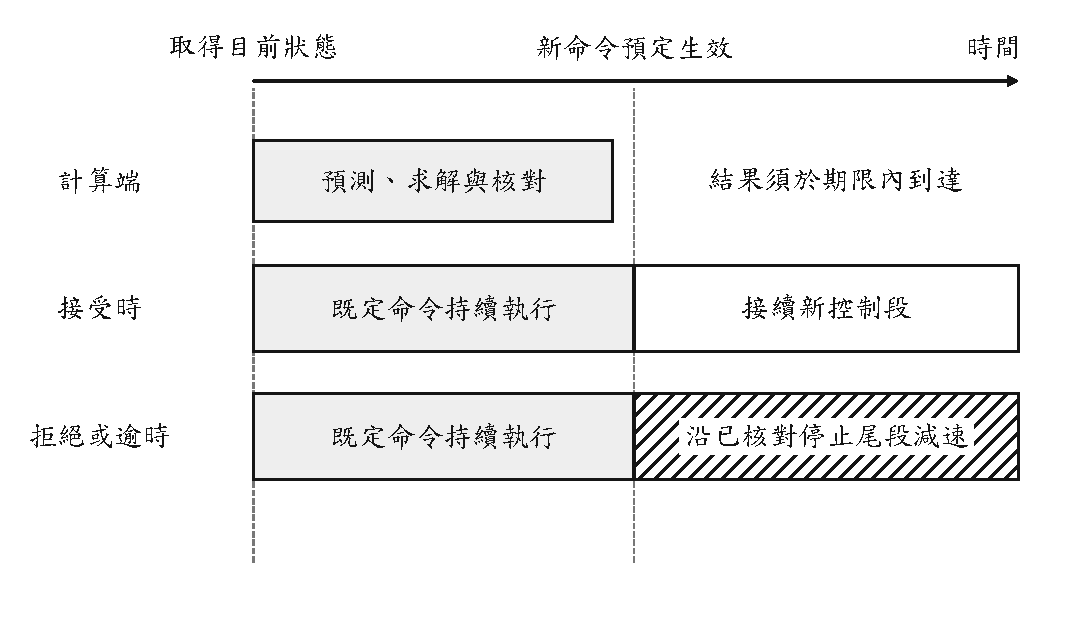
\includegraphics[width=0.98\textwidth]{figsrc/ch03/command_execution_timeline.pdf}
    \caption{控制計算期間之命令接續與停止備援}
    \label{fig:ch3_command_execution_timeline}
\end{figure}

% ==================================================
% 3.7.2 模型偏置估測與末端追蹤補償
% ==================================================
\subsection{模型偏置估測與末端追蹤補償}
\label{subsec:model_bias_tcp_compensation}

手臂模型中的每步偏置 $b_a$ 可表示為 $b_a=D_\alpha d_a$，其中 $d_a$ 為等效關節偏移。令 $B_\ell=\operatorname{diag}(\beta_1^\ell,\ldots,\beta_6^\ell)$，$\Lambda_m=I_6-B_m$。對包含 $m$ 個物理步的完整量測區間，使用更新前的估計 $\hat d_a^{-}$ 與逐步實際生效設定點 $\tilde s_a^{j+\ell}$ 預測：
\begin{equation}
    \hat q_a^{j+m,-}
    =B_m q_a^j
     +\sum_{\ell=0}^{m-1}
       B_{m-1-\ell}D_\alpha\tilde s_a^{j+\ell}
     +\Lambda_m\hat d_a^{-}.
    \label{eq:ch3_interval_offset_prediction}
\end{equation}
其中 $\tilde s_a$ 依其實際作用區間重新對齊，與第 3.2 節的取樣定義一致，不能只依訊息到達順序配對。

由區間終點殘差得到偏移觀測與平滑更新：
\begin{equation}
    \begin{aligned}
        d_a^{\mathrm{obs}}
        &=\hat d_a^{-}
          +\Lambda_m^{-1}
            (q_a^{j+m}-\hat q_a^{j+m,-}),\\
        \hat d_a^{+}
        &=\Pi_{\mathcal D}
          \left[
             \hat d_a^{-}
             +\lambda_d(d_a^{\mathrm{obs}}-\hat d_a^{-})
          \right],\\
        \lambda_d&=\frac{m\Delta t_p}{\tau_d},
        \qquad 0<\lambda_d\leq1,\\
        \hat b_a&=D_\alpha\hat d_a^{+}.
    \end{aligned}
    \label{eq:ch3_interval_offset_update}
\end{equation}
其中 $\Pi_{\mathcal D}$ 為容許範圍投影，包含絕對偏移及相對初始值的修正上限。僅在資料完整、數值有限及區間長度符合設定時更新，同一快照只使用一次。評估殘差以更新前估計計算，保留其對後續預測的檢驗意義。

啟用此估測的接近階段，在閉爪開始後凍結估計，並依配置承接至機構操作。更新後的偏置由 QP 預測、在途命令前推與停止軌跡核對共用。此偏移描述指定區間內的等效追蹤差異，其物理來源可能包含負載、伺服追蹤與模型近似。

% ==================================================
% 3.7.2 模型偏置估測之區間殘差與共用模型更新
% ==================================================
模型偏置估測的更新位置如\cref{fig:ch3_model_bias_estimation}所示。區間末殘差先由更新前的偏置估計計算，經平滑與限幅後，再將新偏置提供給後續 QP 預測、在途命令前推與停止軌跡核對使用。

\begin{figure}[htbp]
    \centering
    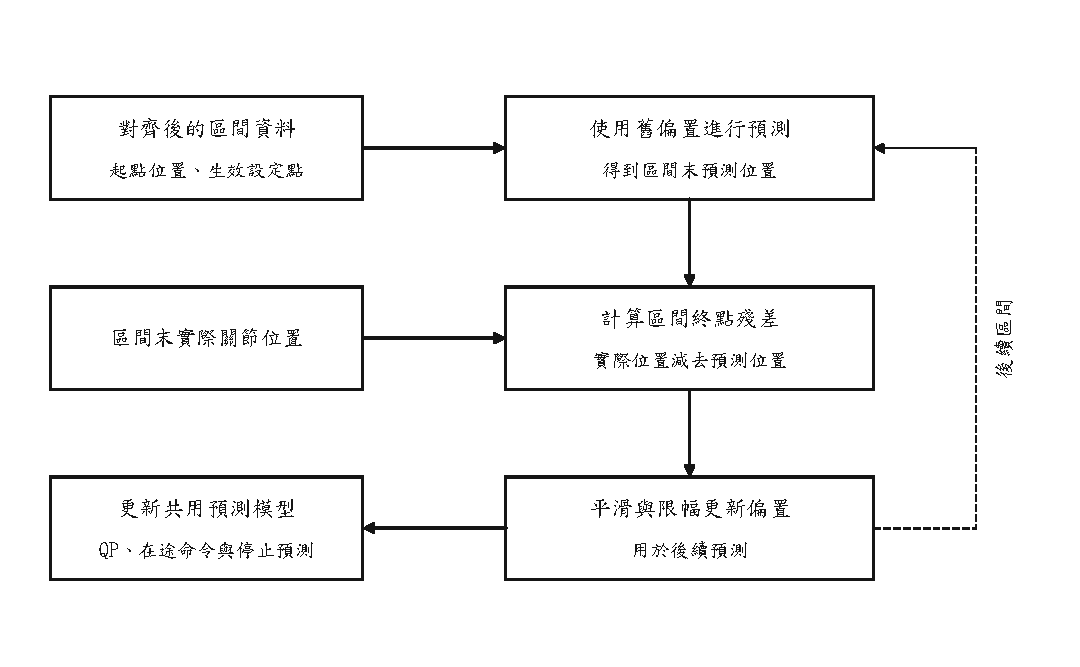
\includegraphics[width=0.98\textwidth]{figsrc/ch03/model_bias_estimation.pdf}
    \caption{模型偏置估測之區間殘差與共用模型更新}
    \label{fig:ch3_model_bias_estimation}
\end{figure}

此外，接近末段可對 TCP 的持續位置誤差施加有界積分補償。令 $\iota_k$ 為目標修正量，在符合接近進度、誤差及低 TCP 速度條件時，更新
\begin{equation}
    \begin{aligned}
        e_{p,k}&=p_{E,k}^{d}-p_{E,k},\\
        \iota_{k+1}
        &=\operatorname{clip}
          (\iota_k+K_I^{d}e_{p,k},-\bar\iota,\bar\iota),\\
        p_{E,k}^{d,\mathrm{cmd}}
        &=p_{E,k}^{d}+\iota_k.
    \end{aligned}
    \label{eq:ch3_bounded_tcp_target_compensation}
\end{equation}
其中 $K_I^{d}$ 為每次更新的離散增益，$\bar\iota$ 為逐軸修正上限。未滿足更新條件時保持補償量，閉爪與確認期間依配置凍結。控制器使用修正後目標產生命令，完成與否仍對原始幾何目標判定。

% ==================================================
% 3.7.2 末端原始幾何目標與有界命令目標補償
% ==================================================
末端目標修正的作用如\cref{fig:ch3_tcp_target_compensation}所示。圖中以單一位置分量說明原始幾何目標、實際末端位置及補償後命令目標的差異；補償量只改變控制器追蹤的命令目標，完成條件仍以原始幾何目標判定。

\begin{figure}[htbp]
    \centering
    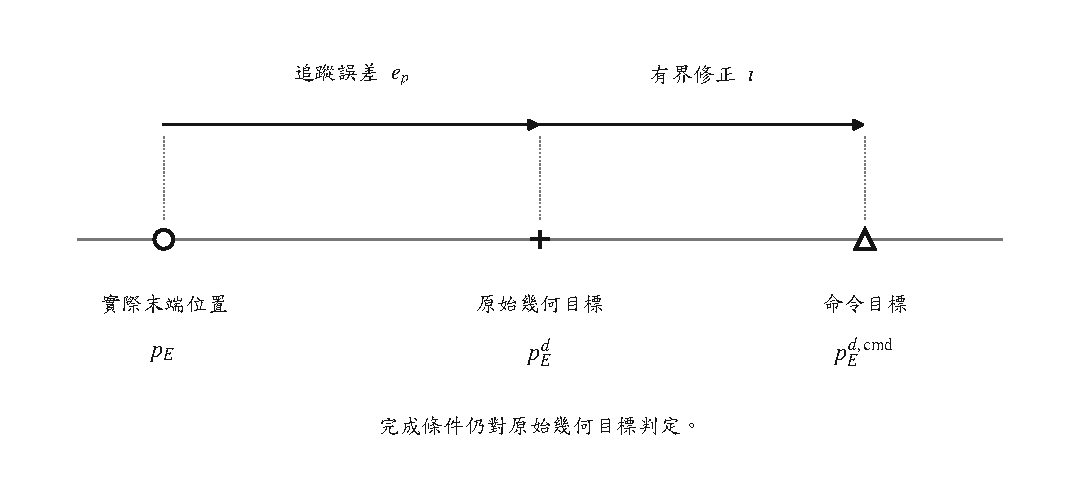
\includegraphics[width=0.98\textwidth]{figsrc/ch03/tcp_target_compensation.pdf}
    \caption{末端原始幾何目標與有界命令目標補償}
    \label{fig:ch3_tcp_target_compensation}
\end{figure}

模型偏置估測改變關節狀態轉移，TCP 補償則改變追蹤目標，兩者的作用位置、啟用階段及消融比較分別記錄。


% ==================================================
% 3.7.3 命令放行、停止軌跡檢查與逾時處置
% ==================================================
\subsection{命令放行、停止軌跡檢查與逾時處置}
\label{subsec:command_acceptance_stopping}

控制計算與平台更新採非阻塞方式執行。求解端根據狀態快照產生帶有版本、預定生效步與控制段的候選封包，平台在計算期間繼續執行已接受的控制段。新結果須在對應期限內到達，並於指定生效步通過版本、狀態及交接檢查後才放行。

候選命令除接受 QP 與命令界限核對外，另沿同一套可執行停止策略前推。停止預測保留在途命令、底盤命令斜坡、輪級變化限制及手臂設定點動態，並依任務納入門角、抽屜開度及持物幾何。對選定取樣步 $\mathcal I_{\mathrm{stop}}$，核對
\begin{equation}
    \begin{aligned}
        q_{\min}&\leq q_{a,\ell}^{\mathrm{stop}}\leq q_{\max},\\
        s_{\min}&\leq s_{a,\ell}^{\mathrm{stop}}\leq s_{\max},\\
        d_{\mathrm{geom},\ell}&\geq d_{\min},\\
        \mathcal G_{\mathrm{contact},\ell}&=1,
        \qquad \ell\in\mathcal I_{\mathrm{stop}}.
    \end{aligned}
    \label{eq:ch3_stopping_trajectory_checks}
\end{equation}
其中 $d_{\mathrm{geom},\ell}$ 包含啟用的環境、自碰撞及持物淨空，$\mathcal G_{\mathrm{contact},\ell}$ 為該階段需要維持的機構或抓持條件；無對應接觸任務時取一。取樣密度、外形近似與容許量依實驗配置揭露。

命令接受條件可概括為
\begin{equation}
    \mathcal G_{\mathrm{accept}}
    =\mathcal G_{\mathrm{ver}}
     \land\mathcal G_{\mathrm{time}}
     \land\mathcal G_{\mathrm{QP}}
     \land\mathcal G_{\mathrm{geom}}
     \land\mathcal G_{\mathrm{handover}},
    \label{eq:ch3_control_packet_acceptance}
\end{equation}
分別表示版本、生效時序與期限、求解及數值檢查、候選與停止軌跡核對，以及適用的任務交接條件。

若候選晚到、求解失敗或未通過檢查，則拒絕該控制段，依已接受的停止尾段減速或進入工程中止。手臂即使令設定點變化率為零，仍可能因 $q_a$ 與 $s_a$ 的差異繼續運動，因此停止核對須前推至設定的停穩條件。新舊控制段的起始狀態、參考與命令亦須檢查接續一致性。

計算池及幾何檢查加速只改變執行方式，各工作使用相同幾何快照與判準。控制期限、牆鐘耗時及模擬時間分別統計，並於第四章分析接受率、逾時原因與適用限制。


% ==================================================
% 3.7.4 整體控制流程與演算法
% ==================================================
\subsection{整體控制流程與演算法}
\label{subsec:overall_control_algorithm}

整體方法以任務階段更新參考與限制，以共用模型預測底盤及手臂運動，再由執行端核對與回授形成閉迴路。

整體控制流程如\cref{fig:ch3_wholebody_control_workflow}所示。系統由狀態與感知更新開始，建立生效起點與任務參考後求解全身 GMPC，再依候選核對結果執行新控制段或停止備援，最後以實際命令與新狀態形成回授。

\begin{figure}[htbp]
    \centering
    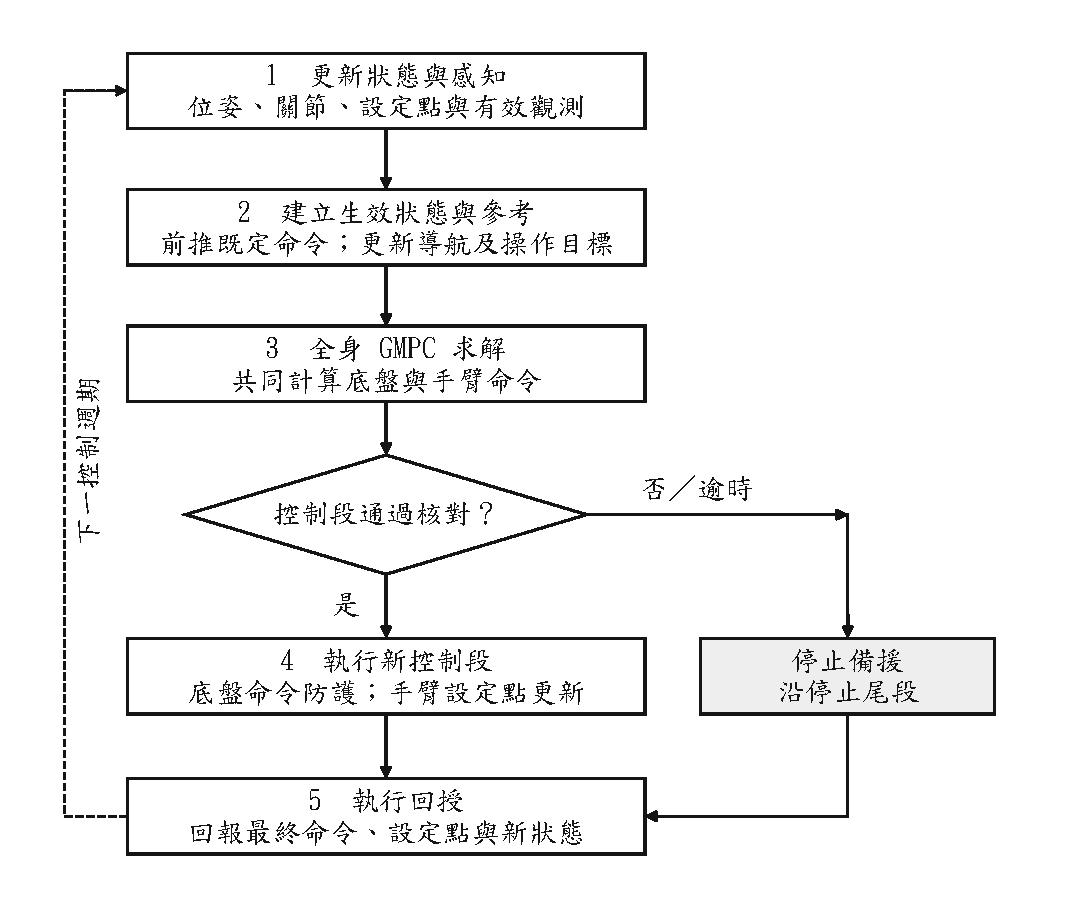
\includegraphics[width=0.98\textwidth]{figsrc/ch03/wholebody_control_workflow.pdf}
    \caption{全身預測控制之計算、命令核對與執行回授流程}
    \label{fig:ch3_wholebody_control_workflow}
\end{figure}

每一控制週期的運作如下：

\begin{enumerate}
    \item 取得機器人位姿、關節位置、位置設定點、障礙與視覺資料，保留來源時間及序號，檢查資料有效性。
    \item 使用完整量測區間更新允許啟用的模型偏置估測，再依已排定命令前推至新控制段的生效起點。
    \item 更新任務階段、操作目標與可行底盤候選；依導航路徑產生接近、抓持、機構操作或持物參考。
    \item 預測動態障礙並評估速度與偏移候選，更新導航參考及對應速度；依任務啟用範圍處理門區與操作限制。
    \item 建立增廣預測、末端局部近似及目標函數，加入命令、關節、輪級、CBF 與適用的機構限制後求解。
    \item 核對求解結果、候選控制段及停止尾段，將合格結果連同版本與生效步提交執行端。
    \item 於指定時刻判定是否接受新控制段；執行後回報最終放行命令、設定點及任務事件，未通過時沿既定停止策略處理。
\end{enumerate}

透過上述流程，導航參考、操作目標與執行模型可在同一控制迴圈中更新。第三章建立各方法及其實現關係；實際使用的版本、參數、比較條件與結果，於第四章依模型預測、動態導航、協同操作及整合任務分別驗證。
